\documentclass[conference]{IEEEtran}
\IEEEoverridecommandlockouts
\usepackage{cite}
\usepackage{amsmath,amssymb,amsfonts}
\usepackage{algorithmic}
\usepackage{graphicx}
\usepackage{textcomp}
\usepackage{xcolor}
\usepackage{xurl} % Permite saltos de línea automáticos e impecables en URLs largas
\usepackage{hyperref}
\usepackage{float}
\def\BibTeX{{\rm B\kern-.05em{\sc i\kern-.025em b}\kern-.08em
    T\kern-.1667em\lower.7ex\hbox{E}\kern-.125emX}}

\begin{document}

\title{SheetMusic: Modelo Computacional de Aprendizaje Adaptativo para la Enseñanza de Teoría Musical mediante un Grafo de Conocimiento y Deep Reinforcement Learning}

\author{
\IEEEauthorblockN{Vicente Alves}
\IEEEauthorblockA{
\textit{Escuela de Ingeniería Civil en Informática} \\
\textit{Universidad Austral de Chile}\\
Valdivia, Chile \\
vicente.alves@alumnos.uach.cl}
\and
\IEEEauthorblockN{Fernando Inzulza}
\IEEEauthorblockA{
\textit{Escuela de Ingeniería Civil en Informática} \\
\textit{Universidad Austral de Chile}\\
Valdivia, Chile \\
fernando.inzulza@alumnos.uach.cl}
\and
\IEEEauthorblockN{Luis Veas-Castillo}
\IEEEauthorblockA{
\textit{Instituto de Informática} \\
\textit{Universidad Austral de Chile}\\
Valdivia, Chile \\
luis.veasc@inf.uach.cl}
\and
\IEEEauthorblockN{Christian Lazo}
\IEEEauthorblockA{
\textit{Instituto de Informática} \\
\textit{Universidad Austral de Chile}\\
Valdivia, Chile \\
clazo@inf.uach.cl}
\and
\IEEEauthorblockN{Abel Mansilla}
\IEEEauthorblockA{
\textit{Facultad de Arquitectura y Artes}\\
\textit{Universidad Austral de Chile}\\
Valdivia, Chile\\
abel.mansilla@uach.cl}
\and
}

\maketitle

\begin{abstract}
La enseñanza de la teoría musical en el contexto escolar enfrenta desafíos derivados de la reducción de la carga horaria, la discontinuidad curricular y la heterogeneidad en los conocimientos previos de los estudiantes. Aunque existen diversas plataformas digitales de apoyo al aprendizaje musical, estas presentan una limitada capacidad para adaptar las actividades según el progreso individual y representar explícitamente las dependencias entre los contenidos.

Este trabajo propone un \textbf{modelo de aprendizaje adaptativo} que integra un \textbf{Grafo de Conocimiento Dirigido Acíclico (DAG)} para representar las dependencias pedagógicas entre conceptos de teoría musical y un agente basado en \textbf{Deep Reinforcement Learning (DRL)} para recomendar dinámicamente la siguiente actividad de aprendizaje de acuerdo con el estado de conocimiento de cada estudiante.

El modelo fue implementado mediante \textbf{SheetMusic}, una plataforma web progresiva orientada al aprendizaje adaptativo y al seguimiento pedagógico de los estudiantes. La validación experimental consideró una prueba piloto de 28 días con 28 estudiantes y una evaluación de usabilidad y aceptación tecnológica con docentes de la Región de Los Ríos, Chile.

Los resultados muestran una mejora aproximada del \textbf{20\%} en la mediana del nivel de \textit{proficiency} de los estudiantes, junto con una alta usabilidad (\textbf{SUS = 82.5/100}) y una favorable aceptación tecnológica (\textbf{TAM = 3.75/5} en utilidad percibida y \textbf{4.00/5} en facilidad de uso). Estos resultados evidencian que la integración de un Grafo de Conocimiento con \textbf{Deep Reinforcement Learning} constituye una estrategia efectiva para implementar modelos computacionales de aprendizaje adaptativo en teoría musical.


\end{abstract}

\begin{IEEEkeywords}
Aprendizaje Adaptativo, Deep Reinforcement Learning, Grafo de Conocimiento, Recomendación Adaptativa, Teoría Musical, Sistemas Inteligentes Educativos.
%Aprendizaje Adaptativo, Educación Musical, Servicio Web, Deep Reinforcement Learning, Grafos de Conocimiento, Usabilidad, TAM.
\end{IEEEkeywords}

\section{INTRODUCCIÓN}

La formación musical escolar desempeña un rol fundamental en el desarrollo cognitivo, creativo y crítico de los estudiantes. Sin embargo, durante las últimas décadas la enseñanza de la música en Chile ha experimentado una progresiva reducción de su presencia dentro del currículo escolar. Decretos ministeriales como el N.\textsuperscript{o} 2960 y el N.\textsuperscript{o} 628 disminuyen la carga horaria destinada a la asignatura a medida que los estudiantes avanzan en su trayectoria escolar, obligando a compartir horas con Artes Visuales o relegando la música a un plan electivo en los niveles superiores~\cite{mineduc_decreto2960_2012, mineduc_decreto628_2016}.

Esta disminución de la carga horaria ha generado dos problemas relevantes para el proceso de enseñanza-aprendizaje de la teoría musical:

\begin{enumerate}
\item \textbf{Discontinuidad curricular y heterogeneidad del aprendizaje.} La reducción de horas y la falta de continuidad en los programas provocan que los estudiantes lleguen a cursos superiores con importantes diferencias en sus conocimientos musicales, dificultando el trabajo del docente y el desarrollo de actividades homogéneas dentro del aula~\cite{chandia_educacion_2025}.

\item \textbf{Limitada disponibilidad de herramientas adaptativas para el contexto escolar.} Aunque existen plataformas digitales orientadas al aprendizaje musical, como Yousician o Simply Piano, estas han sido diseñadas principalmente para contextos de autoaprendizaje, presentan escasa alineación con el currículo escolar chileno y utilizan rutas de aprendizaje predominantemente lineales, sin considerar explícitamente las dependencias pedagógicas entre los contenidos ni las necesidades particulares de cada estudiante~\cite{garcia2025, alrowais2025, li2025}.
\end{enumerate}

Como consecuencia, los docentes deben enfrentar cursos con niveles de conocimiento altamente heterogéneos, mientras que las herramientas tecnológicas disponibles ofrecen una capacidad limitada para adaptar dinámicamente las actividades de aprendizaje según el progreso individual de cada estudiante. Esta situación evidencia la necesidad de modelos computacionales capaces de representar explícitamente la estructura del dominio de conocimiento y utilizar dicha representación para personalizar el proceso de enseñanza.

En este contexto surge la siguiente pregunta de investigación:

\begin{quote}
\textit{¿Cómo desarrollar un modelo computacional de aprendizaje adaptativo capaz de recomendar dinámicamente actividades de teoría musical de acuerdo con el progreso del estudiante y la estructura pedagógica del dominio?}
\end{quote}

Se plantea como hipótesis que la integración de una representación explícita del conocimiento pedagógico con un modelo basado en \textit{Deep Reinforcement Learning} (DRL) permite generar recomendaciones personalizadas que mejoran el proceso de aprendizaje de teoría musical, ajustando dinámicamente la secuencia de actividades de acuerdo con el progreso individual del estudiante y las dependencias existentes entre los contenidos~\cite{sutton2018reinforcement,mnih2015dqn}.

Para validar esta hipótesis se desarrolló \textbf{SheetMusic}, una plataforma que implementa el modelo propuesto mediante la integración de un Grafo de Conocimiento Dirigido Acíclico (DAG) y un agente basado en \textit{Deep Reinforcement Learning}, encargado de recomendar dinámicamente la siguiente actividad de aprendizaje de acuerdo con el progreso del estudiante. La plataforma incorpora además herramientas de seguimiento pedagógico para el docente.

Las principales contribuciones de este trabajo son las siguientes:

\begin{itemize}
\item La formalización del dominio de teoría musical mediante un Grafo de Conocimiento Dirigido Acíclico que representa explícitamente las dependencias pedagógicas entre los contenidos.

\item El desarrollo de un modelo de aprendizaje adaptativo basado en \textit{Deep Reinforcement Learning}, capaz de recomendar dinámicamente actividades de acuerdo con el estado de aprendizaje de cada estudiante.

\item La implementación del modelo en la plataforma \textbf{SheetMusic}, integrando el motor inteligente dentro de una arquitectura distribuida orientada al aprendizaje adaptativo.

\item La validación experimental del modelo mediante una prueba piloto realizada con estudiantes y docentes de la Región de Los Ríos, evaluando tanto el desempeño del modelo adaptativo como la percepción de usabilidad y aceptación tecnológica de la plataforma.
\end{itemize}

El resto del artículo se organiza de la siguiente manera. La Sección II presenta los trabajos relacionados y el estado del arte. La Sección III describe el modelo propuesto y la arquitectura de la plataforma \textbf{SheetMusic}. La Sección IV presenta la validación experimental y los resultados obtenidos. Finalmente, la Sección V expone las conclusiones y las principales líneas de trabajo futuro.

\section{TRABAJOS RELACIONADOS Y ESTADO DEL ARTE}

El aprendizaje adaptativo en teoría musical integra conceptos de educación musical, inteligencia artificial y sistemas inteligentes. Esta sección revisa las principales plataformas existentes, los avances recientes en representación del conocimiento y aprendizaje adaptativo, y la brecha científica que motiva este trabajo.

\subsection{Plataformas de Aprendizaje Musical}

En el ámbito comercial y de acceso abierto destacan plataformas como \textit{Yousician}, \textit{Simply Piano}, \textit{Teoria.com} y \textit{Duolingo Music}. Estas herramientas han contribuido significativamente a masificar el acceso al aprendizaje musical mediante experiencias gamificadas e interfaces interactivas. Sin embargo, presentan diversas limitaciones para su incorporación como herramientas de apoyo en el contexto escolar:

\begin{itemize}

\item \textbf{Alineación curricular e idioma:} La mayoría de estas plataformas fueron desarrolladas para mercados angloparlantes y no se encuentran alineadas con las bases curriculares del sistema educativo chileno ni latinoamericano~\cite{garcia2025,alrowais2025}.

\item \textbf{Apoyo al proceso docente:} Su diseño está orientado principalmente al autoaprendizaje, careciendo de mecanismos que permitan al profesor monitorear el progreso de los estudiantes, identificar brechas de aprendizaje o asignar actividades diferenciadas~\cite{garcia2025,alrowais2025,li2025}.

\item \textbf{Secuencias de aprendizaje rígidas:} Generalmente organizan los contenidos mediante rutas de aprendizaje predefinidas o predominantemente lineales, limitando la personalización del recorrido formativo y la incorporación de representaciones explícitas de las dependencias pedagógicas entre los contenidos~\cite{alrowais2025,li2025}.

\end{itemize}

\subsection{Representación del Conocimiento y Aprendizaje Adaptativo}

La representación explícita del dominio de conocimiento constituye un componente fundamental en los sistemas de aprendizaje adaptativo, ya que permite modelar las relaciones de dependencia entre conceptos, definir prerrequisitos y estructurar trayectorias de aprendizaje coherentes~\cite{manrique2019kg}. En el dominio de la teoría musical, esta representación resulta especialmente relevante debido a la naturaleza progresiva de los contenidos, donde la comprensión de conceptos avanzados depende del dominio previo de conocimientos fundamentales.

Paralelamente, la incorporación de técnicas de Inteligencia Artificial en educación ha experimentado un importante crecimiento durante los últimos años. En el ámbito de la educación musical, diversos trabajos han explorado el uso de IA para la generación automática de contenidos, entrenamiento auditivo y evaluación del desempeño de los estudiantes~\cite{garcia2025}.

Particularmente, el \textit{Deep Reinforcement Learning} (DRL) ha demostrado ser una alternativa efectiva para resolver problemas de decisión secuencial y personalización del aprendizaje, permitiendo aprender políticas de recomendación adaptativas a partir de la interacción con el entorno~\cite{sutton2018reinforcement,mnih2015dqn}. Entre los algoritmos más utilizados destacan \textit{Deep Q-Network} (DQN) y \textit{Proximal Policy Optimization} (PPO), ampliamente empleados para el aprendizaje de políticas en problemas de decisión secuencial. En educación, estos enfoques han sido utilizados para optimizar trayectorias de aprendizaje considerando el desempeño y la evolución individual de cada estudiante~\cite{alrowais2025,li2025}.

No obstante, en el dominio de la educación musical la mayor parte de las investigaciones se han concentrado en composición asistida por IA, entrenamiento auditivo o herramientas de apoyo institucional. Asimismo, las investigaciones revisadas no consideran simultáneamente una representación explícita del conocimiento disciplinar y un mecanismo de decisión basado en aprendizaje por refuerzo para recomendar trayectorias de aprendizaje adaptativas.

\subsection{Brecha Científica}

Del análisis del estado del arte se observa que las soluciones existentes abordan parcialmente el problema del aprendizaje adaptativo. Mientras las plataformas comerciales proporcionan experiencias de aprendizaje gamificadas, los trabajos de investigación exploran la utilización de técnicas de inteligencia artificial para personalizar el proceso educativo. Sin embargo, no se identifican propuestas que integren simultáneamente:

\begin{enumerate}

\item Una representación explícita del conocimiento de teoría musical que modele las dependencias pedagógicas entre los contenidos.

\item Un modelo basado en \textit{Deep Reinforcement Learning} capaz de recomendar dinámicamente la siguiente actividad de aprendizaje de acuerdo con el progreso del estudiante.

\item Una plataforma que permita implementar dicho modelo en un entorno real, incorporando además herramientas de seguimiento pedagógico para el docente.

\end{enumerate}

Esta brecha evidencia la necesidad de integrar representación explícita del conocimiento y aprendizaje por refuerzo para recomendar dinámicamente actividades de teoría musical de acuerdo con el progreso del estudiante.

\section{SOLUCIÓN PROPUESTA}

La solución propuesta consiste en un modelo computacional de aprendizaje adaptativo para la enseñanza de teoría musical, diseñado para recomendar dinámicamente actividades de acuerdo con el progreso individual del estudiante y la estructura pedagógica del dominio. El modelo integra tres componentes principales: (i) un Grafo de Conocimiento Dirigido Acíclico (DAG), encargado de representar explícitamente las dependencias entre los conceptos musicales; (ii) un agente basado en \textit{Deep Reinforcement Learning} (DRL), responsable de aprender una política de recomendación adaptativa; y (iii) la plataforma \textbf{SheetMusic}, que implementa el modelo y proporciona las funcionalidades de interacción para estudiantes y docentes.

La Figura~\ref{fig:modelo_conceptual} presenta una visión conceptual de la propuesta. En ella, el Grafo de Conocimiento define las dependencias pedagógicas que restringen el espacio de decisión del agente basado en DRL, mientras que el estado del estudiante proporciona el contexto utilizado para generar la siguiente recomendación adaptativa. El resultado de la actividad seleccionada retroalimenta el estado del estudiante, completando un ciclo continuo de aprendizaje personalizado implementado por la plataforma \textbf{SheetMusic}.

\begin{figure}[htbp]
    \centering
    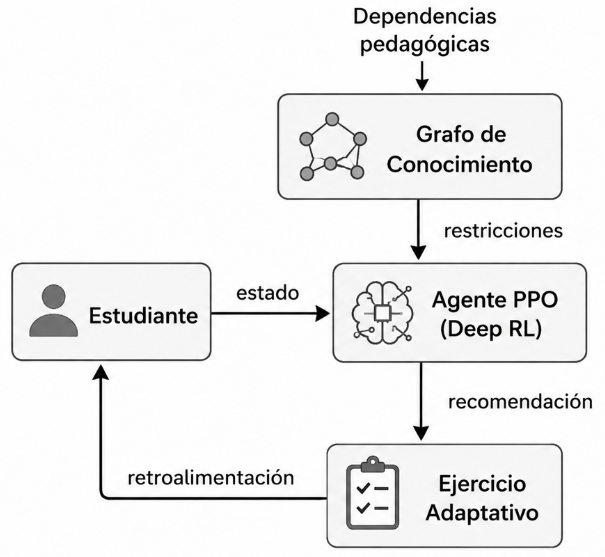
\includegraphics[width=0.26\textwidth]{Imagenes/modelo_conceptual.png}
    \caption{Modelo conceptual del sistema de recomendación adaptativa propuesto.}
    \label{fig:modelo_conceptual}
\end{figure}

A partir de esta visión general, las siguientes subsecciones describen el modelo funcional de la plataforma, la representación del dominio mediante el Grafo de Conocimiento Musical, el modelo de recomendación basado en \textit{Deep Reinforcement Learning} y la arquitectura distribuida utilizada para su implementación.
%--------------------------------------------------------
\subsection{Modelo Funcional de SheetMusic}

La plataforma \textbf{SheetMusic} implementa el modelo de aprendizaje adaptativo mediante dos actores principales: el estudiante, responsable del proceso de aprendizaje, y el profesor, encargado del seguimiento pedagógico. La Figura~\ref{fig:casos_uso} resume las funcionalidades disponibles para ambos perfiles y establece el contexto funcional sobre el cual opera el modelo propuesto.

\begin{figure}[htbp]
    \centering
    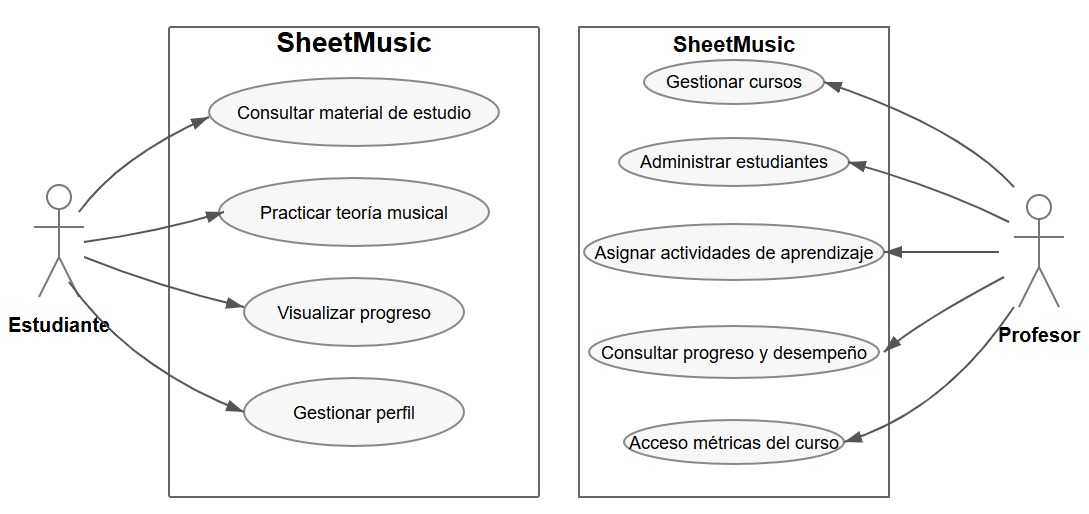
\includegraphics[width=0.36\textwidth]{Imagenes/caso_uso.jpeg}
    \caption{Modelo funcional de la plataforma SheetMusic, mostrando los principales casos de uso para los perfiles de Estudiante y Profesor.}
    \label{fig:casos_uso}
\end{figure}

%--------------------------------------------------------
\subsection{Grafo de Conocimiento Musical}

El dominio de teoría musical se formalizó mediante un Grafo de Conocimiento Dirigido Acíclico (DAG), definido como:

\begin{equation}
G=(V,E)
\end{equation}

donde $V$ representa el conjunto de unidades de conocimiento y $E$ las relaciones de dependencia pedagógica entre ellas.

En la implementación completa, el DAG está compuesto por 23 unidades de conocimiento distribuidas en cinco niveles y 29 relaciones de dependencia pedagógica. Estas relaciones representan prerrequisitos recomendados, permitiendo flexibilizar la progresión cuando el estudiante demuestra un dominio suficiente de los contenidos.

Para la validación experimental se utilizó un subgrafo compuesto por cuatro unidades fundamentales: \textit{Notas y Ritmo}, \textit{Intervalos}, \textit{Escalas Mayores y Menores} y \textit{Acordes (Tríadas)}, suficiente para evaluar el comportamiento del sistema.

\begin{figure}[htbp]
    \centering
    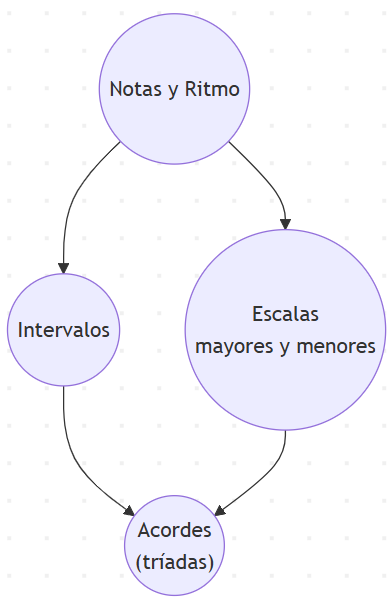
\includegraphics[width=0.15\textwidth]{Imagenes/grafo_dag.png}
    \caption{Subgrafo del Grafo de Conocimiento Musical utilizado durante la validación experimental.}
    \label{fig:dag}
\end{figure}

Cada nodo mantiene un estado asociado al progreso del estudiante, definido mediante:

\begin{equation}
State(v_i)=
\begin{cases}
\text{locked}, & \exists u \in Pred(v_i)\mid Prog(u)\neq\text{done}\\
\text{done}, & Prog(v_i)=\text{done}\\
\text{active}, & Prog(v_i)=\text{in\_progress}\\
\text{available}, & \text{en otro caso}
\end{cases}
\end{equation}

El DAG define el conjunto de actividades pedagógicamente válidas para cada estado del estudiante y constituye el espacio de decisión sobre el cual opera el agente basado en \textit{Deep Reinforcement Learning}. De esta forma, las recomendaciones generadas consideran simultáneamente el estado de aprendizaje del estudiante y las relaciones de dependencia existentes entre los conceptos musicales.

%--------------------------------------------------------
\subsection{Modelo de Recomendación Basado en Deep Reinforcement Learning}

Una vez representado el dominio de conocimiento mediante el Grafo de Conocimiento Musical, el problema de recomendación adaptativa se modela como un proceso de decisión secuencial, donde un agente basado en \textit{Deep Reinforcement Learning} (DRL) selecciona dinámicamente la siguiente actividad de aprendizaje considerando el estado actual del estudiante y las restricciones pedagógicas definidas por el DAG. El objetivo del agente consiste en aprender una política de recomendación que maximice el progreso esperado del estudiante, equilibrando la consolidación de conocimientos, la exploración de nuevos contenidos y la dificultad de los ejercicios.

La implementación del agente se desarrolló utilizando \textit{Stable-Baselines3} (versión 2.0.1) sobre \textit{Gymnasium} (versión 1.2.0), siguiendo el esquema clásico de interacción \textit{agent-environment loop}, donde el agente observa el estado del estudiante, selecciona una actividad, recibe retroalimentación y actualiza iterativamente su política de decisión.

\subsubsection{Entorno de Aprendizaje}

El entorno \texttt{MusicLearningEnv}, implementado como una subclase de \texttt{gymnasium.Env}, modela la interacción entre el agente y el estudiante, donde cada episodio corresponde a la resolución de un ejercicio.

\subsubsection{Espacio de Observaciones}

El estado del estudiante se representa mediante la clase \texttt{UserState}, la cual integra variables asociadas al nivel de dominio de los conceptos, desempeño histórico, dificultad de los ejercicios y evolución reciente del aprendizaje. Para el proceso de inferencia, el nivel de dominio se discretiza utilizando un umbral de proficiencia de 0.5:

\begin{equation}
o_i=
\begin{cases}
1, & \text{si } proficiency_i \ge 0.5\\
0, & \text{en otro caso}
\end{cases}
\end{equation}

obteniendo un vector \texttt{MultiBinary(N)} que representa el estado utilizado por el agente DRL durante la inferencia.

\subsubsection{Espacio de Acciones}

El espacio de acciones corresponde a un conjunto discreto \texttt{Discrete(N)}, donde cada acción representa un ejercicio asociado a un nodo del DAG mediante \texttt{skill\_mapping}, permitiendo incorporar nuevos contenidos sin modificar la estructura del agente.

\subsubsection{Función de Recompensa}

La política del agente se aprende mediante la maximización de una recompensa acumulada que refleja el equilibrio entre el progreso pedagógico del estudiante y la calidad de las recomendaciones generadas. Para ello, se definió una función de recompensa compuesta por incentivos y penalizaciones, orientada a favorecer trayectorias de aprendizaje efectivas y evitar decisiones pedagógicamente inadecuadas.

\begin{equation}
\begin{aligned}
R =\;&
1.0\,\mathbb{I}(\text{correcto})
+0.5\,\mathbb{I}(\text{mejoría}) \\
&+0.5\,\mathbb{I}\!\left(
|d-d^{*}|\le1
\right)
-0.3\,\mathbb{I}\!\left(
|d-d^{*}|>2
\right) \\
&+0.2\,\mathbb{I}(\text{nodo poco practicado})
+0.1\,\mathbb{I}(\text{ejercicio nuevo})
\end{aligned}
\end{equation}

donde $d^{*}=proficiency\times10$ representa la dificultad esperada para el nivel actual del estudiante.

Los términos positivos incentivan respuestas correctas, mejoras respecto al desempeño previo, ejercicios cercanos a la zona de desarrollo proximal, exploración de contenidos poco practicados y variedad en las actividades recomendadas. Por otra parte, el agente recibe penalizaciones cuando recomienda ejercicios cuya dificultad resulta inadecuada para el nivel del estudiante, cuando repite innecesariamente un mismo ejercicio o cuando intenta acceder a contenidos cuyos prerrequisitos pedagógicos definidos por el DAG aún no han sido alcanzados. En consecuencia, el agente aprende simultáneamente a maximizar el progreso esperado del estudiante y a minimizar recomendaciones pedagógicamente inconsistentes.

\subsubsection{Selección del Algoritmo de Aprendizaje}

Con el objetivo de seleccionar el algoritmo más adecuado para el problema de recomendación adaptativa, se compararon dos enfoques ampliamente utilizados en \textit{Deep Reinforcement Learning}: \textit{Deep Q-Network} (DQN) \cite{mnih2015dqn} y \textit{Proximal Policy Optimization} (PPO) \cite{schulman2017ppo}.

Durante las pruebas experimentales, DQN presentó una convergencia inicial más rápida, mientras que PPO desarrolló políticas más estables y un mejor equilibrio entre exploración y explotación. Además, su arquitectura \textit{actor-critic} y el uso de políticas estocásticas permitieron generar recomendaciones más consistentes con la variabilidad esperada en procesos de aprendizaje adaptativo.

Considerando que, en un contexto educativo, la estabilidad de la política de recomendación resulta más importante que una convergencia acelerada, se seleccionó PPO como motor de recomendación del sistema, ya que permite generar trayectorias de aprendizaje adaptativas más consistentes con el progreso individual del estudiante.

\subsubsection{Estrategia de Entrenamiento}

Debido a que durante las primeras etapas del proyecto no se disponía de datos históricos de interacción suficientes para entrenar el agente mediante aprendizaje por refuerzo, se diseñó una estrategia de entrenamiento en dos etapas.

Inicialmente se aplicó un cuestionario a estudiantes de enseñanza media para estimar perfiles de conocimiento y parámetros de aprendizaje. A partir de esta información se implementó el simulador probabilístico \texttt{SyntheticStudent}, encargado de generar trayectorias sintéticas de aprendizaje.

El entrenamiento siguió un esquema híbrido. En una primera etapa se aplicó \textit{Behavior Cloning}, técnica de aprendizaje por imitación utilizada para inicializar una política a partir de criterios pedagógicos definidos por expertos~\cite{osa2018imitation}. Posteriormente, esta política fue refinada mediante \textit{Proximal Policy Optimization} (PPO) utilizando aproximadamente 200\,000 interacciones simuladas.

Este enfoque combina conocimiento pedagógico explícito con la capacidad de optimización del \textit{Deep Reinforcement Learning}, permitiendo que el agente inicie el aprendizaje desde una política consistente y la mejore progresivamente mediante la interacción con el entorno.

%--------------------------------------------------------
\subsection{Arquitectura Distribuida}

La implementación del modelo de aprendizaje adaptativo propuesto se materializa mediante una arquitectura distribuida basada en microservicios, diseñada para desacoplar la interfaz de usuario, la gestión de datos y el motor de inteligencia artificial encargado de generar las recomendaciones adaptativas. Esta separación permite que cada componente evolucione de manera independiente, facilita el escalamiento horizontal del sistema y posibilita incorporar mejoras al modelo de aprendizaje sin modificar la plataforma utilizada por estudiantes y docentes \cite{charland_mobile_2011,flutter_vs_ionic_2023}.

La Figura~\ref{fig:arquitectura} presenta la arquitectura general de \textbf{SheetMusic}, organizada en tres capas principales: una capa cliente responsable de la interacción con los usuarios, una capa de servicios encargada de la autenticación y persistencia de la información académica, y una capa de inteligencia donde se ejecuta el modelo basado en \textit{Deep Reinforcement Learning}.

%--------------------------------------------------------
% FIGURA 3
% Arquitectura General
%--------------------------------------------------------

\begin{figure}[htbp]
    \centering
    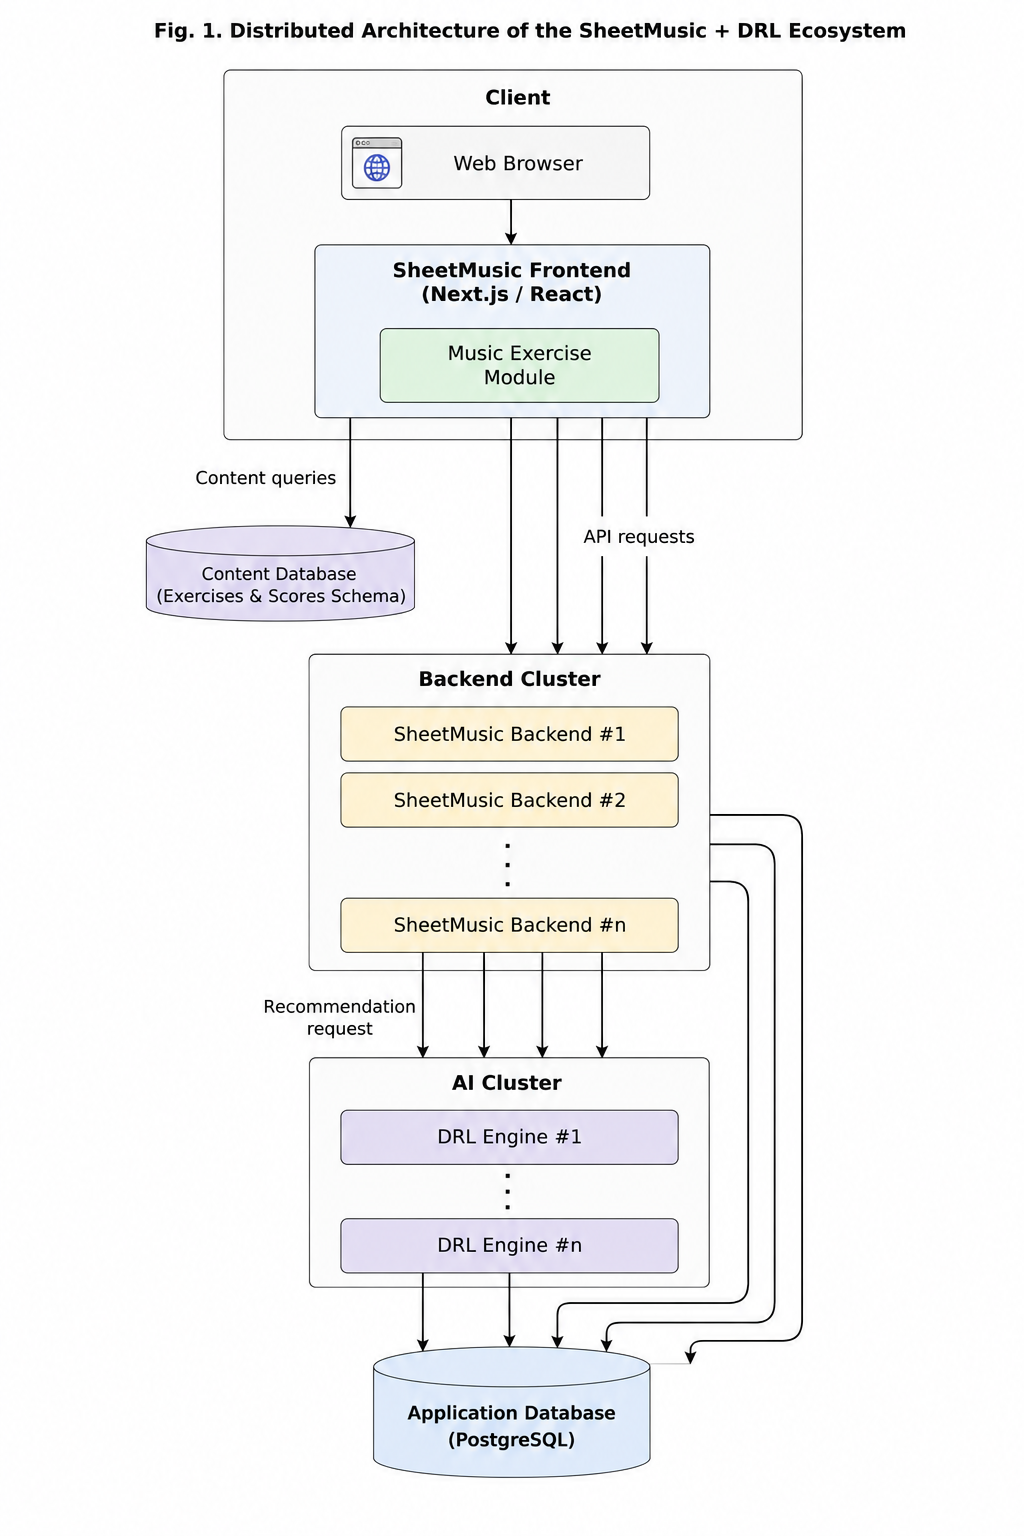
\includegraphics[width=0.3\textwidth]{Imagenes/fig_arch_system.png}
    \caption{Arquitectura distribuida de SheetMusic y sus principales componentes.}
    \label{fig:arquitectura}
\end{figure}

\subsubsection{Componentes de la Arquitectura}

La arquitectura propuesta está compuesta por tres componentes principales:

\begin{itemize}

\item \textbf{Capa Cliente.} Implementada como una \textit{Progressive Web Application} (PWA) utilizando Ionic React y Capacitor, proporciona la interfaz mediante la cual estudiantes y docentes acceden al material de estudio, resuelven ejercicios, consultan su progreso académico y administran las actividades del curso.

\item \textbf{Capa de Servicios.} Implementada sobre Supabase y PostgreSQL, administra la autenticación de usuarios mediante \textit{JSON Web Tokens} (JWT), el almacenamiento del historial académico y la comunicación con la aplicación cliente mediante procedimientos remotos (RPC). Asimismo, aplica políticas de seguridad basadas en \textit{Row Level Security} (RLS), garantizando el aislamiento de la información entre estudiantes y docentes \cite{supabase_docs_2024}.

\item \textbf{Motor de Inteligencia.} Implementado como un microservicio independiente utilizando FastAPI, PyTorch y Stable-Baselines3, recibe el estado actualizado del estudiante, ejecuta el agente basado en PPO y retorna la recomendación del siguiente ejercicio junto con su nivel de dificultad adaptativo.

\end{itemize}

\subsubsection{Flujo de Interacción Distribuida}

La arquitectura implementa dos flujos principales de interacción entre sus componentes. El primero corresponde al acceso al contenido pedagógico y el segundo al proceso de inferencia adaptativa realizado por el agente basado en Deep Reinforcement Learning.

La Figura~\ref{fig:contenido} resume el flujo de renderizado dinámico del contenido pedagógico, desde la solicitud realizada por el cliente hasta la construcción de la interfaz utilizando objetos JSONB recuperados mediante RPC.

%--------------------------------------------------------
% FIGURA 4
%--------------------------------------------------------

\begin{figure}[htbp]
    \centering
    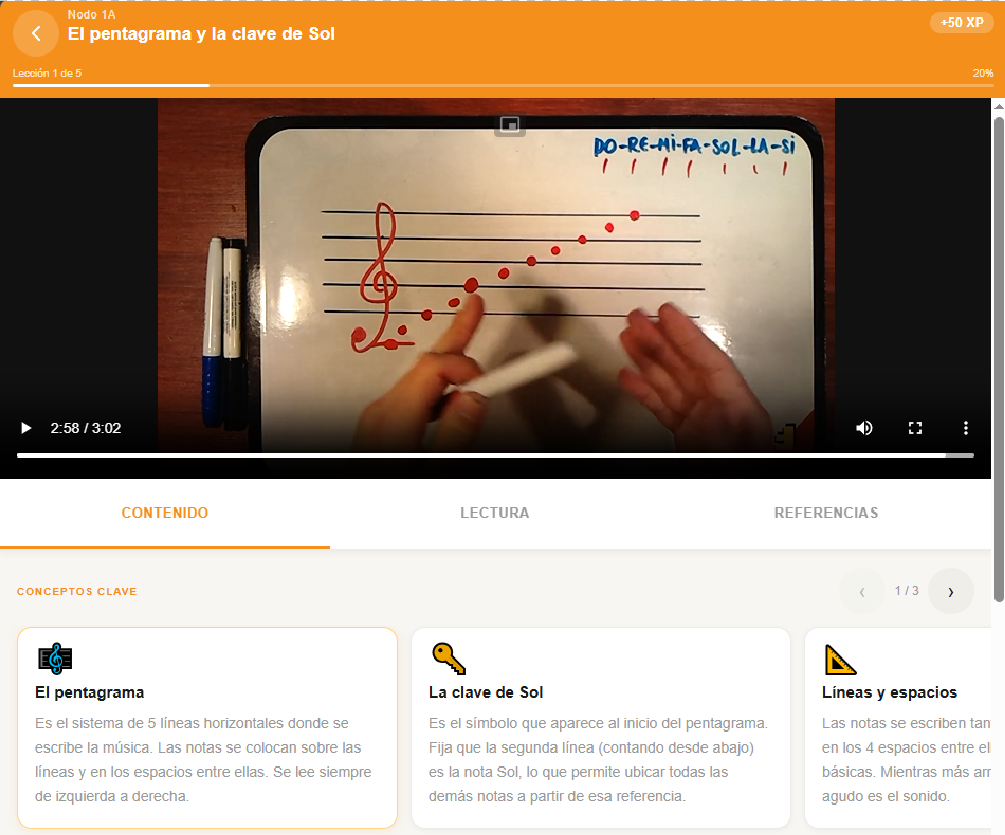
\includegraphics[width=0.3\textwidth]{Imagenes/MaterialAprendizajeFrontend.png}
    \caption{Flujo de renderizado dinámico del contenido pedagógico utilizando objetos JSONB recuperados desde el backend.}
    \label{fig:contenido}
\end{figure}

Una vez finalizada una actividad, se inicia el proceso de recomendación adaptativa mostrado en la Figura~\ref{fig:inferencia}. El cliente envía el resultado del ejercicio al backend, el cual actualiza el estado del estudiante y construye el vector de observaciones utilizado por el agente DRL. Posteriormente, el modelo PPO determina la siguiente recomendación considerando tanto el estado del estudiante como las restricciones definidas por el Grafo de Conocimiento Musical, retornando el ejercicio y su nivel de dificultad adaptativo para completar el ciclo de aprendizaje.

%--------------------------------------------------------
% FIGURA 5
%--------------------------------------------------------

\begin{figure}[htbp]
    \centering
    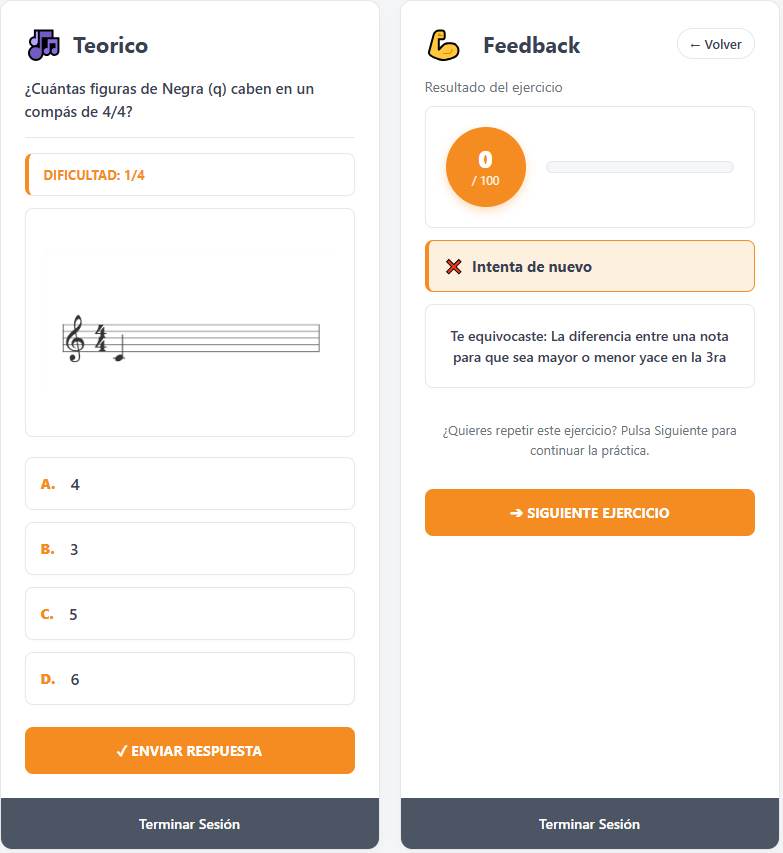
\includegraphics[width=0.3\textwidth]{Imagenes/frontend_ejercicio.png}
    \caption{Flujo distribuido de inferencia entre el cliente, el backend y el motor de Deep Reinforcement Learning.}
    \label{fig:inferencia}
\end{figure}

La arquitectura distribuida propuesta desacopla completamente la representación del conocimiento (DAG), el proceso de toma de decisiones basado en Deep Reinforcement Learning y la interfaz utilizada por estudiantes y docentes. Como consecuencia, nuevas estrategias de recomendación, funciones de recompensa o modelos de aprendizaje pueden incorporarse al sistema sin modificar la plataforma cliente, favoreciendo la mantenibilidad, escalabilidad y evolución futura de \textbf{SheetMusic}.

\section{VALIDACIÓN EXPERIMENTAL}

Con el objetivo de validar la propuesta presentada, se diseñó una evaluación que consideró tanto el desempeño del modelo de aprendizaje adaptativo como la percepción de los usuarios respecto de la plataforma \textbf{SheetMusic}. La validación se estructuró en tres etapas: (i) definición del escenario experimental, (ii) evaluación mediante métricas objetivas y subjetivas, y (iii) análisis de los resultados obtenidos.

%--------------------------------------------------------
\subsection{Diseño Experimental}

La validación se realizó utilizando la versión funcional de \textbf{SheetMusic} desarrollada durante el proyecto. Los participantes interactuaron con la plataforma resolviendo actividades de teoría musical recomendadas por el agente basado en \textit{Deep Reinforcement Learning}. Durante cada sesión se registró automáticamente el estado del estudiante, las recomendaciones realizadas por el sistema y el progreso alcanzado en las distintas unidades de conocimiento.

Finalizada la interacción, estudiantes y docentes respondieron instrumentos estandarizados con el propósito de evaluar la usabilidad y aceptación de la plataforma.

%--------------------------------------------------------
\subsection{Métricas de Evaluación}

La validación experimental consideró dos dimensiones complementarias: (i) el desempeño del modelo de recomendación basado en \textit{Deep Reinforcement Learning} y (ii) la percepción de los usuarios respecto de la plataforma \textbf{SheetMusic}.

\textbf{Evaluación del modelo de recomendación.} Para analizar el comportamiento del agente DRL se utilizaron los siguientes indicadores:

\begin{itemize}

\item \textbf{Progreso de Aprendizaje (Proficiency):} cuantifica el incremento del nivel de dominio alcanzado por el estudiante durante las sesiones de aprendizaje, permitiendo evaluar la efectividad pedagógica de las recomendaciones generadas por el agente.

\item \textbf{Tasa de Continuidad:} mide la permanencia del estudiante en el proceso de aprendizaje mediante el número de sesiones realizadas y la continuidad de uso de la plataforma, proporcionando una estimación indirecta del nivel de compromiso generado por el sistema adaptativo.

\item \textbf{Adaptabilidad de la Dificultad:} evalúa la capacidad del agente para recomendar ejercicios cuya dificultad se mantenga cercana al nivel de competencia del estudiante, evitando tanto la frustración por actividades excesivamente complejas como la pérdida de interés por ejercicios demasiado simples.

\end{itemize}

\textbf{Evaluación de la plataforma.} Para analizar la experiencia de uso de \textbf{SheetMusic} se emplearon instrumentos ampliamente utilizados en la evaluación de sistemas interactivos:

\begin{itemize}

\item \textbf{Usabilidad (SUS):} se aplicó el cuestionario \textit{System Usability Scale (SUS)} para evaluar la facilidad de uso percibida por los estudiantes~\cite{sus_brooke_1996}.

\item \textbf{Aceptación Tecnológica (TAM):} los docentes respondieron un cuestionario basado en el \textit{Technology Acceptance Model (TAM)}, permitiendo evaluar la utilidad percibida, la facilidad de uso y la intención de utilización futura de la plataforma~\cite{davis1989}.

\end{itemize}

%--------------------------------------------------------
\section{RESULTADOS}

La validación consideró 28 estudiantes (5 del Conservatorio de Música de la Universidad Austral de Chile y 23 de enseñanza media de la comuna de Corral), quienes utilizaron SheetMusic durante 28 días consecutivos.

%--------------------------------------------------------
\subsubsection{Resultados del Modelo de Recomendación}

La Figura~\ref{fig:rendimiento_ieee} presenta la evolución del nivel de \textit{proficiency} para tres perfiles representativos de estudiantes: alto, medio y bajo desempeño. En los tres casos se observa una tendencia ascendente, indicando que el agente fue capaz de adaptar progresivamente las recomendaciones al nivel de conocimiento de cada estudiante. Incluso los participantes con menor dominio inicial evidenciaron una mejora sostenida durante el período de evaluación, lo que sugiere que la política aprendida mediante PPO logra personalizar adecuadamente las trayectorias de aprendizaje.

\begin{figure}[htbp]
    \centering
    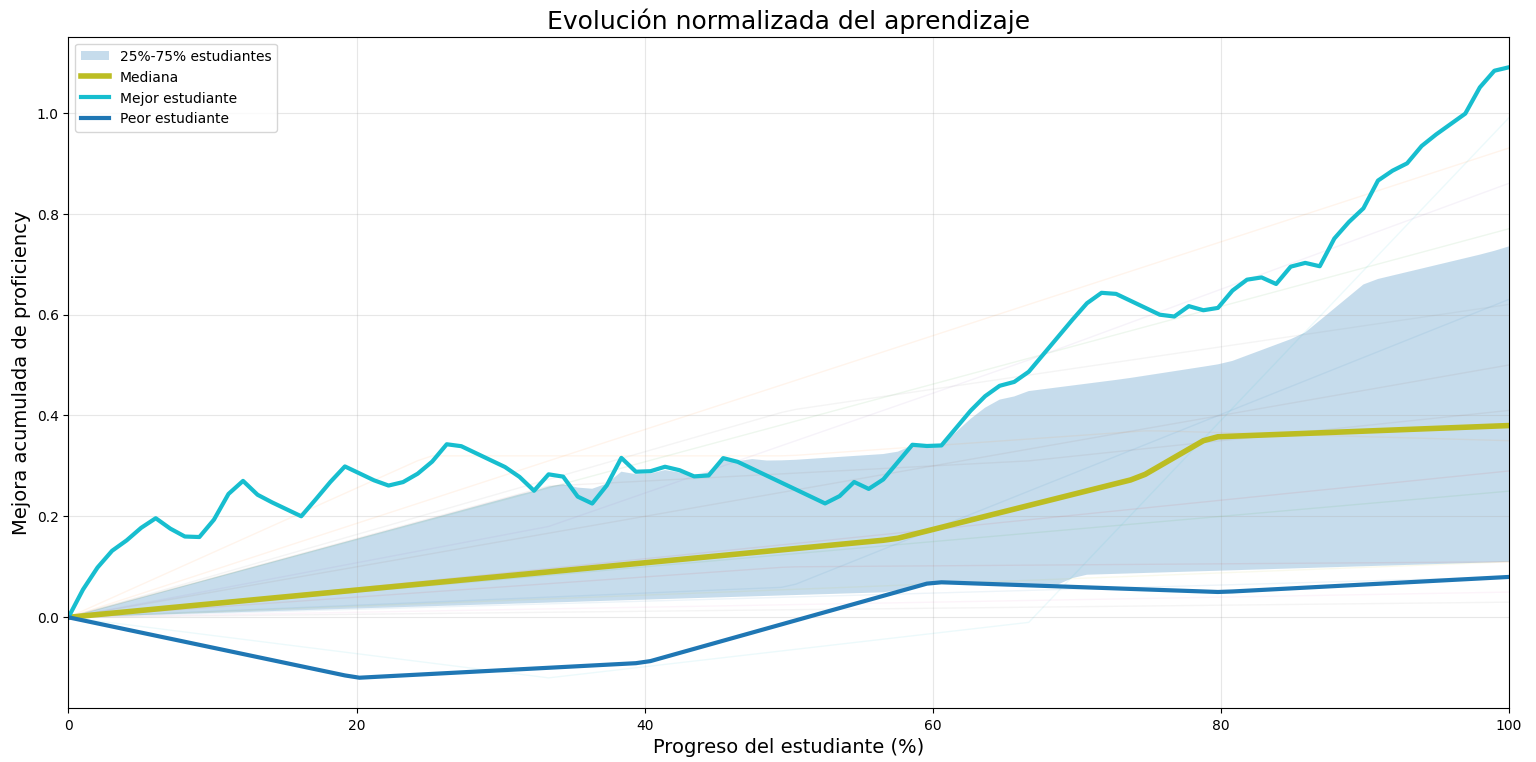
\includegraphics[width=0.45\textwidth]{Imagenes/rendimiento_estudiantes.png}
    \caption{Evolución del nivel de \textit{proficiency} de tres perfiles representativos de estudiantes durante la validación experimental.}
    \label{fig:rendimiento_ieee}
\end{figure}

La continuidad de uso fue evaluada mediante el número de sesiones registradas durante el período experimental. Como se observa en la Figura~\ref{fig:actividad_ieee}, la actividad se mantuvo estable durante las tres primeras semanas de evaluación, acumulando un total de 572 sesiones. La disminución observada durante la cuarta semana corresponde al cierre del proceso de recolección de datos y no a una disminución en el uso de la plataforma.

\begin{figure}[htbp]
    \centering
    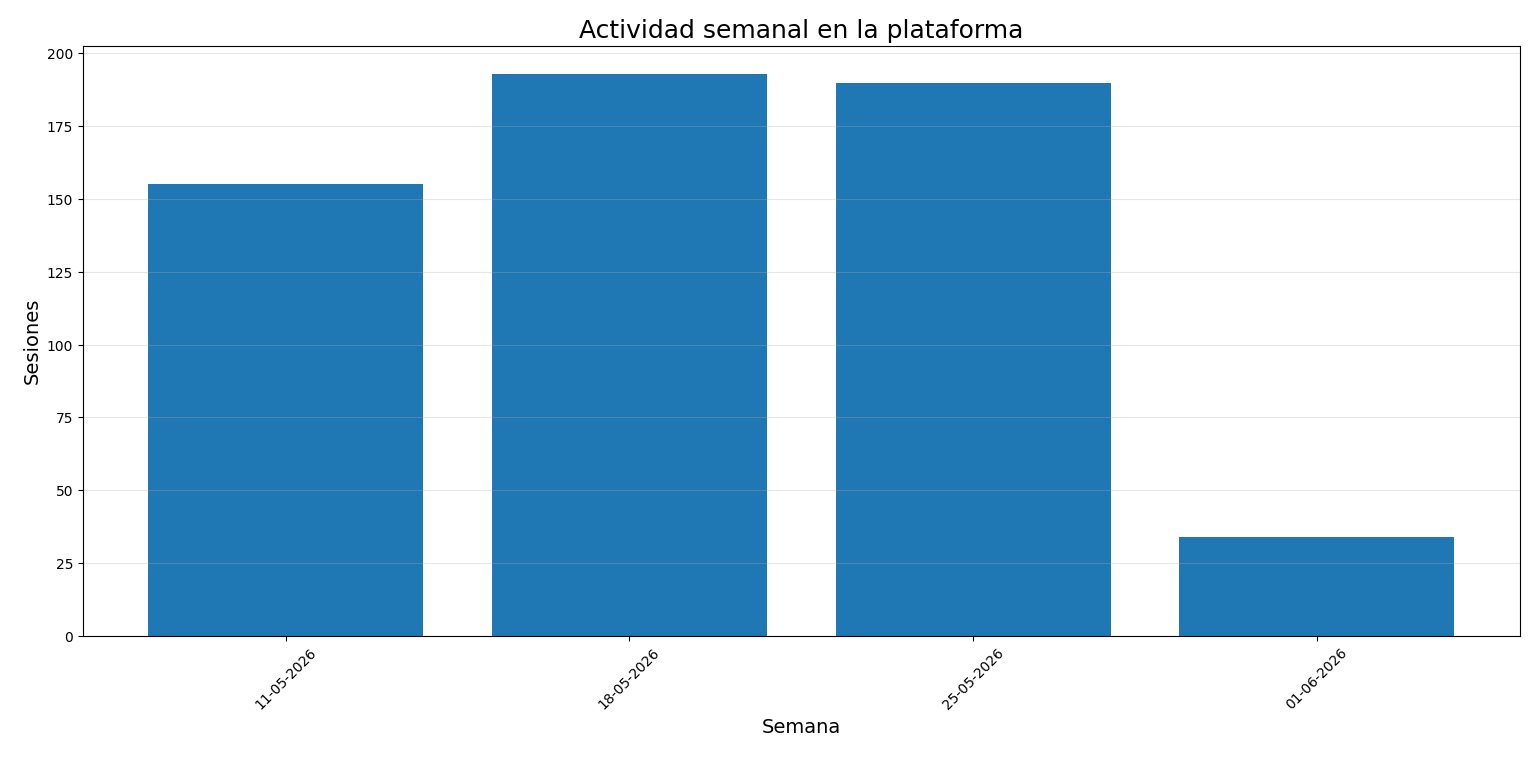
\includegraphics[width=0.45\textwidth]{Imagenes/actividad_semanal.png}
    \caption{Distribución semanal de las sesiones registradas durante el período de validación.}
    \label{fig:actividad_ieee}
\end{figure}

Los principales indicadores obtenidos durante la validación se resumen en la Tabla~\ref{tab:resultados_ieee}. En particular, la mediana del nivel de \textit{proficiency} presentó una mejora aproximada del 20\%, superando la meta inicial del 15\%. Asimismo, el sistema ajustó dinámicamente la dificultad y la secuencia de ejercicios de acuerdo con el desempeño individual de cada estudiante, evidenciando la capacidad del agente DRL para personalizar el proceso de aprendizaje.

\begin{table}[htbp]
\centering
\caption{Resumen de los principales resultados obtenidos durante la validación del modelo de recomendación.}
\label{tab:resultados_ieee}
\begin{tabular}{lp{5.2cm}}
\hline
\textbf{Indicador} & \textbf{Resultado} \\
\hline
Participantes & 28 estudiantes \\
Sesiones registradas & 572 sesiones \\
Continuidad de uso & Actividad sostenida durante el período de evaluación \\
Mejora en \textit{Proficiency} & Incremento aproximado del 20\% (meta: 15\%) \\
Adaptabilidad & Ajuste dinámico de la dificultad y secuencia de ejercicios según el desempeño del estudiante \\
\hline
\end{tabular}
\end{table}

En conjunto, estos resultados indican que el agente basado en \textit{Deep Reinforcement Learning} fue capaz de mantener una progresión positiva del aprendizaje, adaptar las recomendaciones al desempeño individual de los estudiantes y sostener una participación continua durante el período de evaluación.

%--------------------------------------------------------
\subsubsection{Resultados de la Plataforma}

La plataforma \textbf{SheetMusic} fue evaluada mediante los instrumentos \textit{System Usability Scale} (SUS) y \textit{Technology Acceptance Model} (TAM), con el propósito de medir su usabilidad y aceptación tecnológica. Los resultados obtenidos se resumen en la Tabla~\ref{tab:sus_tam}.

\begin{table}[htbp]
\centering
\caption{Resultados de la evaluación de usabilidad y aceptación tecnológica de la plataforma.}
\label{tab:sus_tam}
\begin{tabular}{lc}
\hline
\textbf{Indicador evaluado} & \textbf{Resultado} \\
\hline
Usabilidad (SUS) & 82.5 / 100 \\
TAM -- Utilidad percibida & 3.75 / 5.00 \\
TAM -- Facilidad de uso & 4.00 / 5.00 \\
\hline
\end{tabular}
\end{table}

El puntaje obtenido en SUS indica una percepción positiva respecto de la usabilidad de la plataforma. Asimismo, los resultados del TAM muestran una valoración favorable tanto de la utilidad percibida ($3.75/5.00$) como de la facilidad de uso ($4.00/5.00$), evidenciando una alta aceptación tecnológica por parte de los docentes para incorporar la plataforma como herramienta de apoyo al proceso de enseñanza y aprendizaje.

Los resultados obtenidos complementan la evaluación técnica del modelo de recomendación, mostrando que la propuesta no sólo adapta el proceso de aprendizaje mediante recomendaciones personalizadas, sino que además presenta niveles adecuados de usabilidad y aceptación tecnológica para su utilización en contextos educativos reales. En conjunto, la evidencia obtenida respalda la hipótesis planteada, indicando que la integración de un Grafo de Conocimiento Dirigido Acíclico con un agente basado en \textit{Deep Reinforcement Learning} constituye una estrategia efectiva para implementar aprendizaje adaptativo en teoría musical.

Cabe señalar algunas limitaciones del presente estudio. La validación se realizó sobre una muestra reducida y heterogénea (5 estudiantes de Conservatorio y 23 de enseñanza media), sin grupo de control ni pruebas de significancia estadística, por lo que los resultados constituyen evidencia preliminar sobre el potencial del modelo propuesto. Asimismo, la evaluación consideró únicamente un subgrafo de cuatro unidades de conocimiento (de un total de 23) durante un período de 28 días, por lo que será necesario ampliar tanto la cobertura del dominio como el tamaño y diversidad de la muestra para fortalecer la validez externa de los resultados.

\section{CONCLUSIONES Y TRABAJOS FUTUROS}

En este trabajo se presentó un modelo computacional de aprendizaje adaptativo para la enseñanza de teoría musical, el cual integra un Grafo de Conocimiento Dirigido Acíclico (DAG) para representar explícitamente las dependencias pedagógicas del dominio y un agente basado en \textit{Deep Reinforcement Learning} (DRL) para recomendar dinámicamente actividades de aprendizaje de acuerdo con el progreso individual del estudiante. El modelo fue materializado mediante la plataforma distribuida \textbf{SheetMusic}, permitiendo materializar la propuesta en un entorno real de apoyo al proceso de enseñanza y aprendizaje.

Los resultados obtenidos durante la validación experimental muestran que el agente de recomendación fue capaz de adaptar la secuencia y dificultad de los ejercicios según el desempeño individual de cada estudiante, favoreciendo una progresión sostenida del aprendizaje y manteniendo una participación continua durante el período de evaluación. Asimismo, la evaluación de usabilidad y aceptación tecnológica evidenció una percepción favorable de la plataforma por parte de estudiantes y docentes, respaldando la factibilidad de utilizar este tipo de herramientas como apoyo al aprendizaje de teoría musical en el contexto escolar.

Desde la perspectiva de la Ingeniería Informática, el principal aporte de este trabajo no corresponde únicamente al desarrollo de una plataforma educativa, sino a la definición e implementación de un modelo computacional de aprendizaje adaptativo que integra representación explícita del conocimiento mediante un Grafo de Conocimiento Dirigido Acíclico (DAG) con técnicas de \textit{Deep Reinforcement Learning} para la recomendación personalizada de actividades. Esta integración desacopla la representación del dominio, el proceso de toma de decisiones y la implementación tecnológica, constituyendo una arquitectura reutilizable que puede extenderse a otros dominios educativos donde exista una estructura de conocimiento basada en relaciones de dependencia.

La arquitectura distribuida propuesta facilita además la evolución independiente de sus componentes, permitiendo incorporar nuevos contenidos, estrategias de recomendación o modelos de inteligencia artificial sin modificar la infraestructura principal de \textbf{SheetMusic}. Del mismo modo, el uso de estructuras semiestructuradas basadas en \texttt{JSONB} posibilita ampliar el contenido pedagógico y los recursos multimedia de forma flexible, favoreciendo la mantenibilidad y escalabilidad del sistema.

Con el propósito de favorecer la reproducibilidad científica y la continuidad del proyecto, el código fuente de la plataforma, del motor de recomendación y de los microservicios desarrollados se encuentra disponible públicamente en la organización oficial de GitHub: \url{https://github.com/Sheetmusic-Team}.

Como trabajo futuro se contempla ampliar el Grafo de Conocimiento Musical para cubrir la totalidad de las unidades curriculares de teoría musical, incorporar nuevos algoritmos de aprendizaje por refuerzo y comparar su desempeño con PPO, integrar evaluación instrumental en tiempo real mediante procesamiento digital de señales (DSP) y validar la propuesta con una muestra significativamente mayor de estudiantes pertenecientes a distintos establecimientos educacionales. Asimismo, se espera extender el modelo para incorporar nuevos dominios de aprendizaje, evaluando la capacidad de la arquitectura propuesta para reutilizar la representación explícita del conocimiento y el motor de recomendación adaptativa en otros contextos educativos.

\bibliographystyle{IEEEtran}
\bibliography{referencias}

\end{document}